%!TEX TS-program = lualatex
\documentclass[]{friggeri-cv}
\usepackage{afterpage}
\usepackage{hyperref}
\usepackage{color}
\usepackage{xcolor}
\hypersetup{
    pdftitle={},
    pdfauthor={},
    pdfsubject={},
    pdfkeywords={},
    colorlinks=false,       % no lik border color
   allbordercolors=white    % white border color for all
}
\addbibresource{bibliography.bib}
\RequirePackage{xcolor}
\definecolor{pblue}{HTML}{0395DE}

\begin{document}
\header{Arshpreet}     {Singh}
      {Senior Software Engineer}

% Fake text to add separator
\fcolorbox{white}{gray}{\parbox{\dimexpr\textwidth-2\fboxsep-2\fboxrule}{%
.....
}}

% In the aside, each new line forces a line break
\begin{aside}
  \section{Address}
    3159, Sec-40D
    Chandigarh,Punjab, India
    ~
  \section{Tel \& LinkedIn}
    +91 991 5959387
    \href{http://www.linkedin.com/in/arsh840/}{www.linkedin\\.com/in/arsh840/}
    ~
  \section{Mail}
    \href{mailto:arsh840@gmail.com}{\textbf{arsh840@}\\gmail.com}
    ~
  \section{Web \& Git}
    \href{http://www.arshpreetsingh.wordpress.com}{arshpreetsingh.wordpress\\.com}
    \href{https://medium.com/@arshpreetsingh}{https://medium.com/@arshpreet\\singh}
    \href{https://github.com/arshpreetsingh}{github.com/arshpreet\\singh}
    ~
  \section{Programming}
    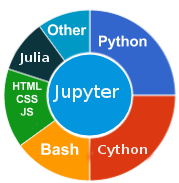
\includegraphics[scale=0.62]{img/programming.png}
    ~
  \section{OS Preference}
    \textbf{GNU/Linux}
\includegraphics[scale=0.40]{img/5stars.png}
    \textbf{Unix}
\includegraphics[scale=0.40]{img/5stars.png}
    \textbf{MacOS}
\includegraphics[scale=0.40]{img/2stars.png}
    \textbf{Windows}
\includegraphics[scale=0.40]{img/2stars.png}
    ~
  \section{Personal Skills}
    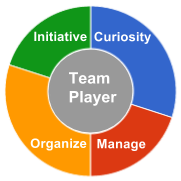
\includegraphics[scale=0.62]{img/personal.png}
    ~
\end{aside}

\section{Experience}
\begin{entrylist}
  \entry
    {01/19 - Now }
    {Senior Software Engineer}
    {Maropost India, Chandigarh}
    {Microservices Development and Deployment using Next Generation Technology Stack, Golang, Protocol Buffers, Kafka, Docker, Kuberbetes and Rancher}
  \entry
    {08/17 - 01/19}
    {Machine Learning Engineer}
    {Exponential Machines}
    {Development of Continuous Intelligence Platform using Python, Flask Web Framework and Machine Learning Libraries like Numpy, Pandas and Scikit learn, Optimzation of Deployment Piplelines using Docker and Rancher. }
   \entry
    {08/17 - 04/18}
    {Senior Software Engineer}
    {Netsmartz Chandigarh}
    {Blockchain POC Creation and Implementation using IBM HyperLedger, Development and Deployment of MicroServices, Automation Testing, Testing Framework Development.}
  \entry
    {05/16 - 10/16}
    {Full-Stack Python Developer}
    {Revinfotech Ludhiana}
    {Design and development of Software Projects using Amazon and Google Clouds, LTSP implementation.Automation of various internal Tasks using Python and Project Management.\\}
    \entry
    {01/14 - 02/15}
    {Linux Trainer and Web Developer}
    {FutureTech IT centre Ludhiana}
    {Teaching Linux Desktop and Server Administration skills to students. Developed various projects using technologies HTML, CSS, JavaScript, Python,
C and shell Script. Computer technical support. Problem solving related to hardware, software and Operating Systems. Management of the internal Structure.\\}
    \entry
    {01/13 - 06/13}
    {Intern-ship}
    {SysInfocom, Chandigarh}
    {Training for Linux Desktop and Server Administration, management and migration of servers. Development of ”Python Battery Saver pack”(Python Based). Learning and using Latex for creating reports and documents.\\}
    \entry
    {06/11 - 07/11}
    {Intern-ship}
    {TCC GNDEC Ludhiana}
    {Training for Python. Worked on college souvenir(Django Based Project).
SageMath Deployment on Server and introduced SageMath and it’s features
to Research Students. Open Source Technologies.\\}
\end{entrylist}
\section{Certifications}
\begin{entrylist}
  \entry
    {07/2019}
    {Go Programming Specialization}
    {Coursera}
    {\emph{}}
  \entry
    {05/2019}
    {Ultimate Go Programming}
    {O'Reilly School of Technology}
    {\emph{}}
  \entry
    {11/2018}
    {Julia Scientific Programming}
    {Coursera}
    {\emph{}}
  \entry
    {09/2018}
    {Deep Learning Specialization}
    {Coursera}
    {\emph{}}
  \entry
    {06/2018}
    {Julia Programming for Scientific Computing}
    {Coursera}
    {\emph{}}
  \entry
    {06/2018}
    {BlockChain Basics and Beyond}
    {Lynda.com}
    {\emph{}}
  \entry
    {12/2016}
    {Python for DataScience and Machine Learning}
    {Udemy. E-learning}
    {\emph{}}
\end{entrylist}

\section{Education}
\begin{entrylist}
  \entry
    {2009 - 2013}
    {Bachelor's Degree in Information Technology}
    {GNDCE Ludhiana,Punjab,India}
    {\emph{}}
  \entry
    {2007 - 2009}
    {Senoir Secondary School}
    {DC Model, Ferozepur}
    {\emph{}}
\end{entrylist}
\begin{aside}
~
~
~
   \section{Languages}
    \textbf{English}
\includegraphics[scale=0.40]{img/4stars.png}
    \textbf{Hindi}
\includegraphics[scale=0.40]{img/5stars.png}
    \textbf{Punjabi}
\includegraphics[scale=0.40]{img/5stars.png}
\end{aside}

\section{Projects}
\begin{entrylist}
 \entry
    {03/2017}
    {Stock prediction using Random Forest}
    {Trading-Algorithm}
    {\emph{www.quantopian.com is used as platform to deploy,benchmark and evaluate performace of the Algorithm for
    single stock.}}
 \entry
    {01/2017}
    {Stock's Analysis using Ensemble Learning}
    {Research work}
    {\emph{Problem Definition: To Predict if close price of day N will be less or more than Close Price of Day N-1.}}
 \entry
    {08/2016}
    {Bitcoin Live Trading using ANN}
    {Revinfotech Ludhiana}
    {\emph{Bitcoin Live Trading is Web-Based System developed Using Django
    Framework.}}
  \entry
    {12/2015}
    {Gmail Analyser}
    {Elance/Upwork}
    {\emph{Gmail Analyser is Flask Based Solution which provides data of All Emails
as per the request.}}
  \entry
    {03/2016}
    {ParaView Advanced Volume Filter}
    {Elance/Upwork}
    {\emph{ParaView is an open-source, multi-platform data analysis and visualization
application.}}
\end{entrylist}

\section{Open-Source Contributions}
\begin{entrylist}
 \entry
    {03/2016}
    {Tuxblocks}
    {Github}
    {\emph{Tuxblocks Game is developed using Java Based PlayN Game Engine.}}

 \entry
    {03/2016}
    {Open Street Mapping}
    {osm.org}
    {\emph{}}

 \entry
    {03/2016}
    {Browser-Based File-Manager}
    {Github}
    {\emph{Flask based File Manager.}}

 \entry
    {03/2016}
    {Text-to-mp3 Android implementation}
    {Github}
    {\emph{Contributed to Open-source project Plyer by creating Python wrapper around
Java Classes.}}


\end{entrylist}


\\
\begin{flushleft}
\emph{July 19th, 2019}
\end{flushleft}
\begin{flushright}
\emph{Arshpreet Singh Khangura}
\end{flushright}
\end{document}
